%!TEX program = lualatex
\documentclass[11pt,class=beamer]{standalone}
\usepackage{etoolbox}
\usepackage{ifxetex}
\usepackage{ifluatex}
\usepackage[T1]{fontenc}
\ifboolexpr{bool{xetex} or bool{luatex}}{%
	\usepackage{fontspec}
}{%
	\usepackage[utf8]{inputenc}
}
\usepackage{xcolor}

\usepackage{amsmath}
\usepackage{amssymb}
\usepackage{mathrsfs}
\usepackage{braket}

\usepackage{pgf}
\usepackage{tikz}
\usepackage{tikzpeople}

\usepackage{array}
\usepackage{tabularx}
\usepackage{multirow}

\usetikzlibrary{shapes}
\usetikzlibrary{arrows.meta}
\usetikzlibrary{calc}
\usetikzlibrary{positioning}
\usetikzlibrary{angles}
\usetikzlibrary{quotes}
\usetikzlibrary{decorations}

\definecolor{bg_color}{RGB}{250,250,229}
\definecolor{Cblue}{RGB}{38,75,150}
\definecolor{Cgreen}{RGB}{39,179,118}
\definecolor{Cdarkgreen}{RGB}{0,111,60}
\definecolor{Corange}{RGB}{249,167,62}
\definecolor{Cred}{RGB}{191,33,47}

\colorlet{good}{green!90!black}
\colorlet{average}{Corange}
\colorlet{bad}{Cred}


\beamertemplatenavigationsymbolsempty{}

\begin{document}
	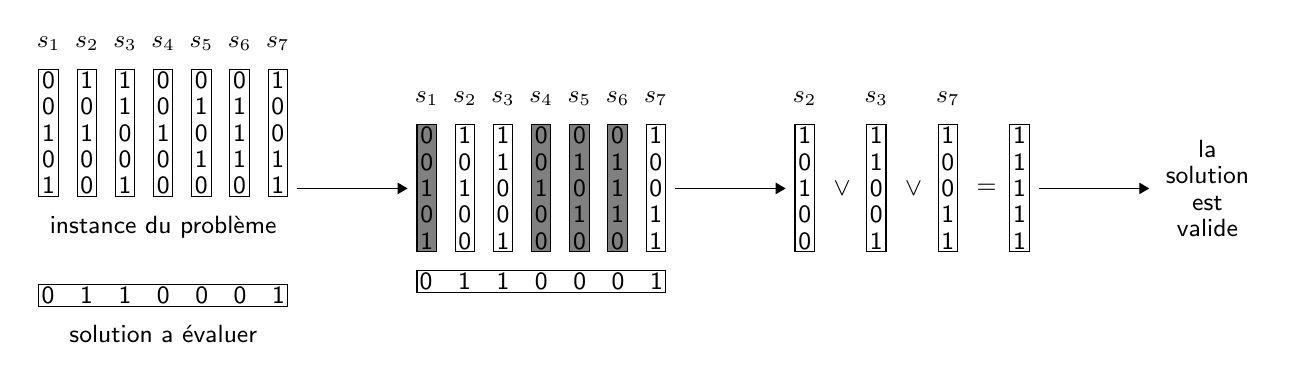
\begin{tikzpicture}[
		x=1pt,
		y=1pt,
		/utils/exec={\sffamily},
		font=\fontsize{9pt}{9.5pt}\selectfont,
		>=Triangle,
		decoration={snake,segment length=5,amplitude=0.7},
	]
		\tikzset{bitset/.style={
			draw,
			rectangle,
			inner sep=1,
			outer sep=3.4,
			text width=5,
			text centered,
		}}
		\tikzset{bitseth/.style={
			draw,
			rectangle,
			inner sep=1,
			outer sep=3.4,
		}}

		%---------------------------------
		% Input
		\node[
			bitset,
			anchor=west,
			xshift=40,
		] (bitset1a) at (0,0) {0\\0\\1\\0\\1};
		\node[
			bitset,
			anchor=west,
		] (bitset2a) at (bitset1a.east) {1\\0\\1\\0\\0};
		\node[
			bitset,
			anchor=west,
		] (bitset3a) at (bitset2a.east) {1\\1\\0\\0\\1};
		\node[
			bitset,
			anchor=west,
		] (bitset4a) at (bitset3a.east) {0\\0\\1\\0\\0};
		\node[
			bitset,
			anchor=west,
		] (bitset5a) at (bitset4a.east) {0\\1\\0\\1\\0};
		\node[
			bitset,
			anchor=west,
		] (bitset6a) at (bitset5a.east) {0\\1\\1\\1\\0};
		\node[
			bitset,
			anchor=west,
		] (bitset7a) at (bitset6a.east) {1\\0\\0\\1\\1};

		\node[anchor=south] at (bitset1a.north) {\(s_1\)};
		\node[anchor=south] at (bitset2a.north) {\(s_2\)};
		\node[anchor=south] at (bitset3a.north) {\(s_3\)};
		\node[anchor=south] at (bitset4a.north) {\(s_4\)};
		\node[anchor=south] at (bitset5a.north) {\(s_5\)};
		\node[anchor=south] at (bitset6a.north) {\(s_6\)};
		\node[anchor=south] at (bitset7a.north) {\(s_7\)};

		\node[
			anchor=north,
		] at (bitset4a.south) {instance du problème};

		\node[
			bitseth,
			anchor=north west,
			yshift=-25,
		] (bitsetxa) at (bitset1a.south west) {0\ \ \ 1\ \ \ 1\ \ \ 0\ \ \ 0\ \ \ 0\ \ \ 1};
		\node[
			anchor=north,
		] at (bitsetxa.south) {solution a évaluer};

		%---------------------------------
		% Selection
		\node[
			bitset,
			anchor=west,
			xshift=40,
			yshift=-20,
			fill=gray,
		] (bitset1b) at (bitset7a.east) {0\\0\\1\\0\\1};
		\node[
			bitset,
			anchor=west,
		] (bitset2b) at (bitset1b.east) {1\\0\\1\\0\\0};
		\node[
			bitset,
			anchor=west,
		] (bitset3b) at (bitset2b.east) {1\\1\\0\\0\\1};
		\node[
			bitset,
			anchor=west,
			fill=gray,
		] (bitset4b) at (bitset3b.east) {0\\0\\1\\0\\0};
		\node[
			bitset,
			anchor=west,
			fill=gray,
		] (bitset5b) at (bitset4b.east) {0\\1\\0\\1\\0};
		\node[
			bitset,
			anchor=west,
			fill=gray,
		] (bitset6b) at (bitset5b.east) {0\\1\\1\\1\\0};
		\node[
			bitset,
			anchor=west,
		] (bitset7b) at (bitset6b.east) {1\\0\\0\\1\\1};

		\node[anchor=south] at (bitset1b.north) {\(s_1\)};
		\node[anchor=south] at (bitset2b.north) {\(s_2\)};
		\node[anchor=south] at (bitset3b.north) {\(s_3\)};
		\node[anchor=south] at (bitset4b.north) {\(s_4\)};
		\node[anchor=south] at (bitset5b.north) {\(s_5\)};
		\node[anchor=south] at (bitset6b.north) {\(s_6\)};
		\node[anchor=south] at (bitset7b.north) {\(s_7\)};

		\node[
			bitseth,
			anchor=north west,
		] (bitsetxb) at (bitset1b.south west) {0\ \ \ 1\ \ \ 1\ \ \ 0\ \ \ 0\ \ \ 0\ \ \ 1};

		\draw[->] (bitset7a.east |- bitset1b) -- (bitset1b);

		%---------------------------------
		% OR
		\node[
			bitset,
			anchor=west,
			xshift=40,
		] (bitset2c) at (bitset7b.east) {1\\0\\1\\0\\0};
		\node[
			anchor=west,
			text width=5,
			text centered,
		] (or1) at (bitset2c.east) {\(\lor\)};
		\node[
			bitset,
			anchor=west,
		] (bitset3c) at (or1.east) {1\\1\\0\\0\\1};
		\node[
			anchor=west,
			text width=5,
			text centered,
		] (or2) at (bitset3c.east) {\(\lor\)};
		\node[
			bitset,
			anchor=west,
		] (bitset7c) at (or2.east) {1\\0\\0\\1\\1};
		\node[
			anchor=west,
			text width=5,
			text centered,
		] (eq) at (bitset7c.east) {\(=\)};
		\node[
			bitset,
			anchor=west,
		] (bitsetrc) at (eq.east) {1\\1\\1\\1\\1};

		\node[anchor=south] at (bitset2c.north) {\(s_2\)};
		\node[anchor=south] at (bitset3c.north) {\(s_3\)};
		\node[anchor=south] at (bitset7c.north) {\(s_7\)};

		\draw[->] (bitset7b) -- (bitset2c);

		%---------------------------------
		% Valid
		\node[
			anchor=west,
			xshift=40,
			text width=35,
			text centered,
		] (valid) at (bitsetrc.east) {la solution est valide};

		\draw[->] (bitsetrc) -- (valid);
	\end{tikzpicture}%
\end{document}%